\begin{savequote}[75mm]
If you can snap two chicken necks in a single motion, why use two motions to slaughter those chickens?
\qauthor{Dwight Schrute}
\end{savequote}

\chapter{Search for Higgs pair production in boosted $\FourB$ final states}
\label{chap:boosted4b}

\section{Introduction}

After the discovery of the Higgs boson in the ATLAS Run 1 dataset and the subsequent measurements of its properties, the Higgs transformed into a potential tool in searches for physics beyond the Standard Model. The pair production cross section of the Higgs can be enhanced through BSM physics. Studying di-Higgs production also probes the Higgs self-coupling, shedding light on the structure of the Higgs potential. This chapter presents a search for resonant production of a Higgs pair in the $\FourBfull$ final state in $3.2 \ifb$ of data collected at $\sqrt{s} = 13 \TeV$. In particular, this chapter focuses on a search for this final state in the regime where $m_{X}$ is large ($\gtrsim 1 \TeV$) and the Higgs bosons in the decay are significantly boosted. A tailored selection for this boosted selection, using novel techniques in jet substructure and $b$-tagging, is discussed. Then, the data-driven background estimate is presented. Finally, the results of the search are shown. Limits on signal models are reserved for the next chapter where the results of this chapter are combined with the results of a separate selection dedicated to the lower $m_X$ regime. 

\section{Motivation}

With the center of mass energy increase from $\sqrt{s} = 8 \TeV$ to $\sqrt{s} = 13 \TeV$, the LHC and ATLAS are able to probe new resonances at higher mass scales than previously accessible in Run 1. This is a powerful motivator for searching for a new resonance in the early $13 \TeV$ data. Figure~\ref{fig:lumi_ratio} shows the ratios of parton luminosities between $8$ and $13 \TeV$ for different resonance masses. For a resonance of $M_{X} = 2 \TeV$, the cross section at $\sqrt{s} = 13 \TeV$ is roughly a factor of $10$ larger than at $\sqrt{s} = 8 \TeV$. 

\begin{figure}[h!]
  %\vspace{20pt}
  \centering
  \captionsetup{justification=centering}

  %\hspace*{-32pt}
  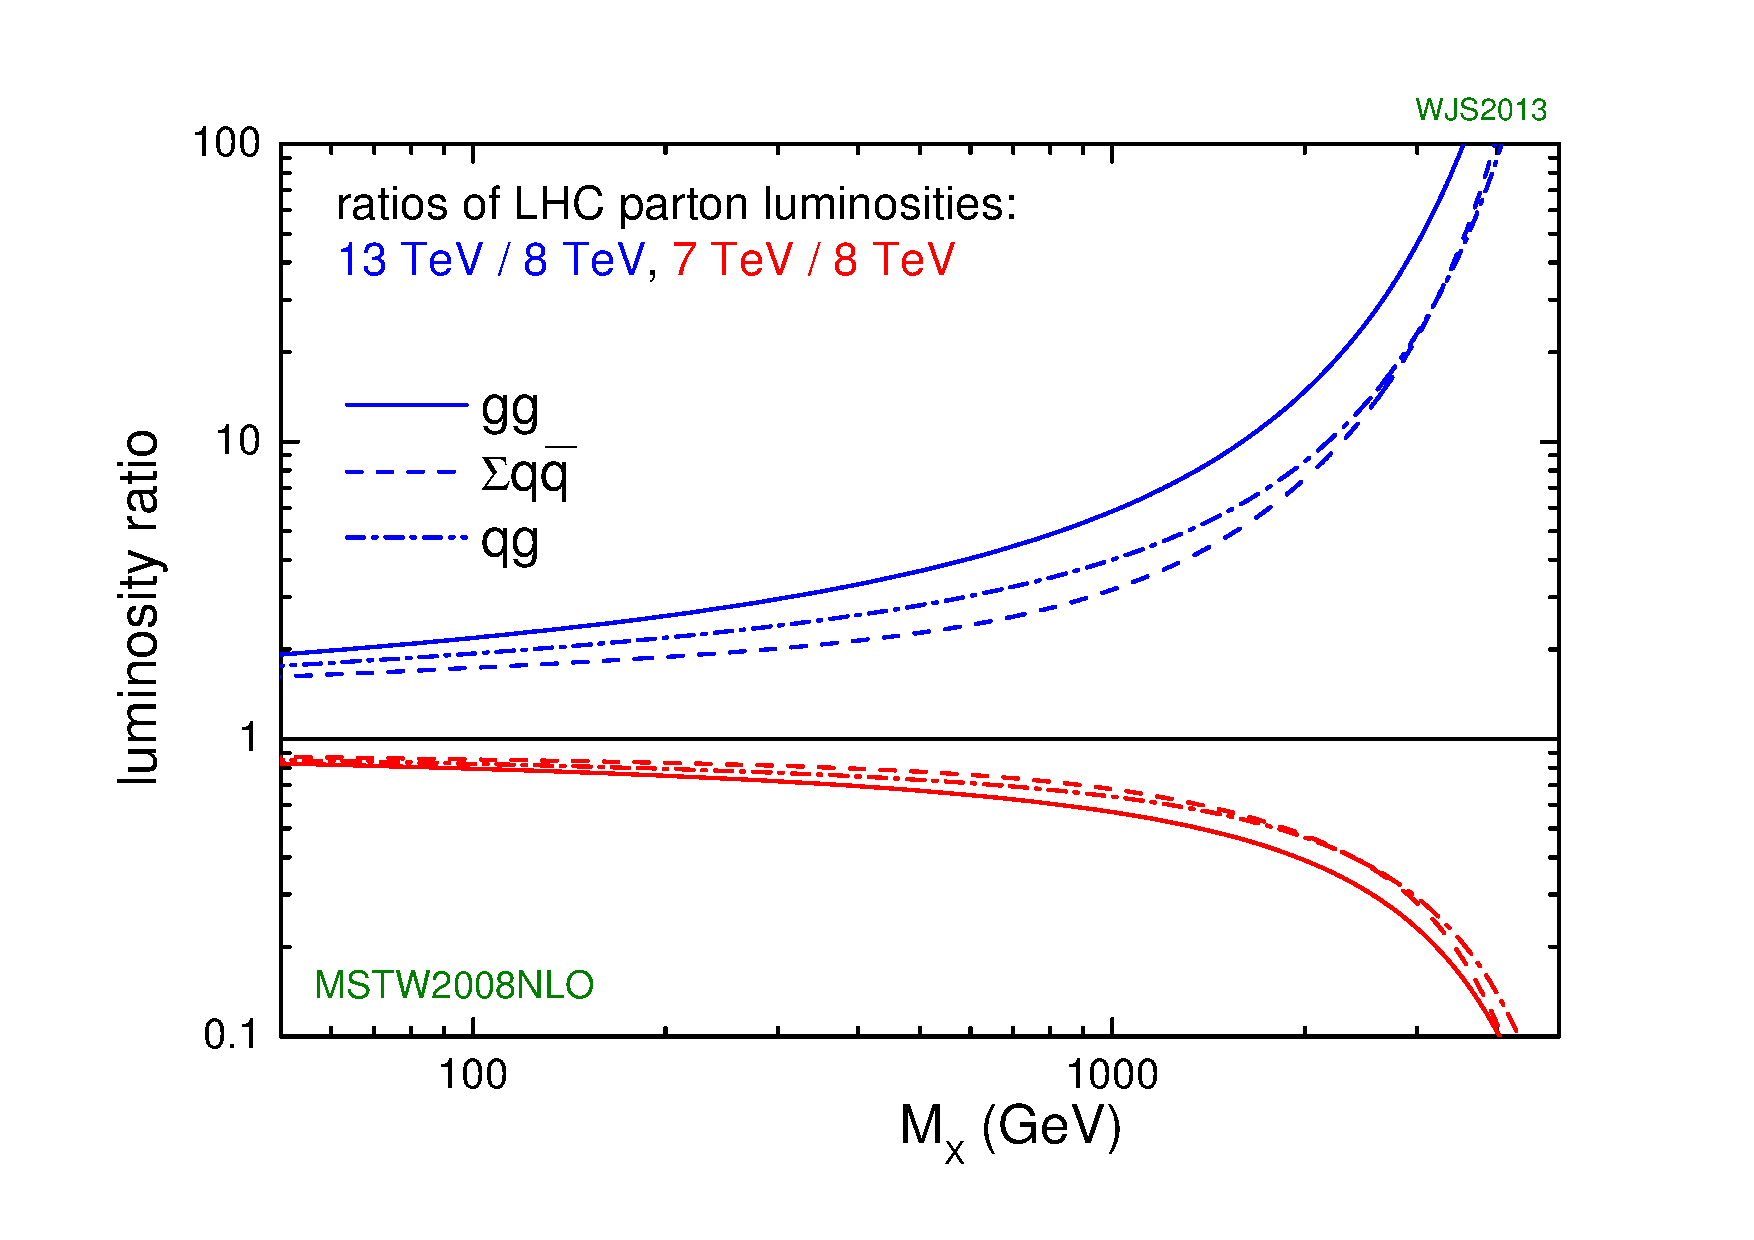
\includegraphics[width=0.6\textwidth,angle=270]{figures/Stirling_lumi_ratios}
  \caption{Parton luminosity ratios as a function of resonance mass $M_{X}$ for $13/8 \TeV$ and $7/8 \TeV$~\cite{LumiRatio}.}
  \label{fig:lumi_ratio}
\end{figure}

Higgs pair production offers a vast array of unprobed regions of phase space where searches for BSM physics can be made. Chapter 1 discusses some possibilities for both resonant and non-resonant enhancement of the di-Higgs production cross section. Given the increased mass reach of the LHC in Run 2, it is particularly important to focus on resonant searches at high $m_{X}$. One consideration when conducting a search in the $HH$ final state is which decay modes of the Higgs to consider. Figure~\ref{fig:HH_BR} shows the branching ratio of the $HH$ final state for different combinations of decays of each individual Higgs. As the largest branching ratio for the $125 \GeV$ Higgs is $H\to b\bar{b}$, the $HH\to b\bar{b}b\bar{b}$ branching ratio is also the largest at $33\%$. 

\begin{figure}[h!]
  %\vspace{20pt}
  \centering
  \captionsetup{justification=centering}

  %\hspace*{-32pt}
  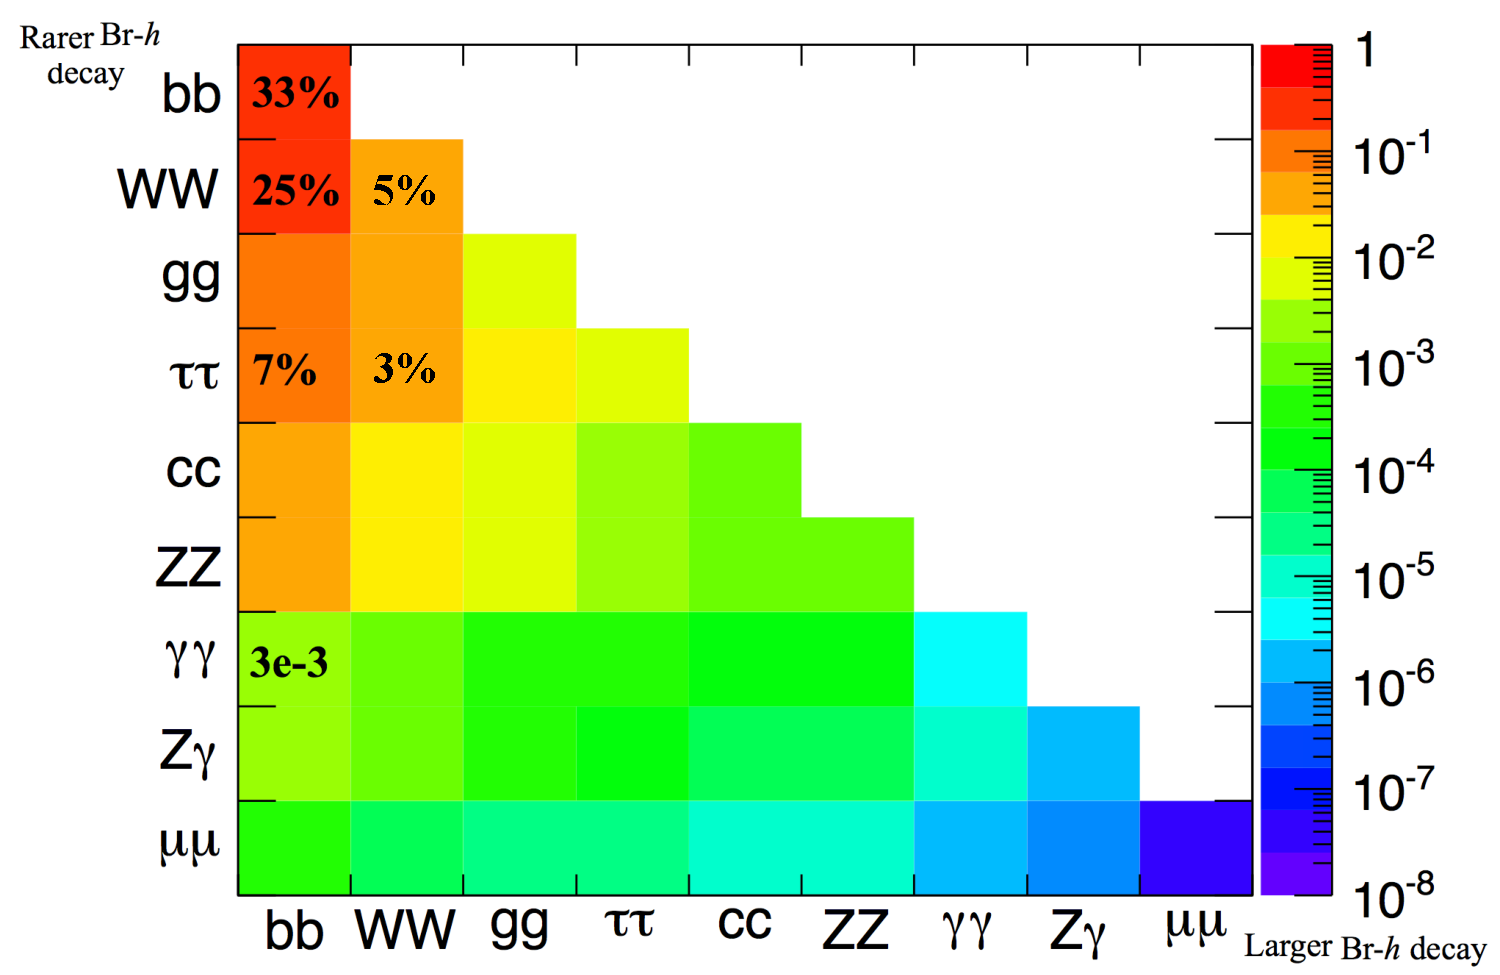
\includegraphics[width=0.8\textwidth]{figures/HH_BR}
  \caption{Summary of $HH$ branching ratios~\cite{HH_BR}.}
  \label{fig:HH_BR}
\end{figure}

\section{Data and simulation samples}

\section{Event reconstruction}

\section{Event selection}

\section{Data-driven background estimation}

\section{Systematic uncertainties}

\section{Results}


